%% ============================================================
%% EJ-204 vs EJ-230 Bar — Full comparative scan
%% 4 configs: TIR-only vs Vikuiti 3M × EJ-204 vs EJ-230
%% Geant4 11.4 MT | rrios / dowiyogo@gmail.com
%% ============================================================
\documentclass[aspectratio=169,10pt]{beamer}

\usetheme{Boadilla}
\usecolortheme{seahorse}
\useinnertheme{circles}
\setbeamertemplate{navigation symbols}{}
\setbeamertemplate{footline}[frame number]

\usepackage[utf8]{inputenc}
\usepackage[T1]{fontenc}
\usepackage{lmodern}
\usepackage{booktabs}
\usepackage{siunitx}
\usepackage{xcolor}
\usepackage{graphicx}
\usepackage{tikz}
\usetikzlibrary{shapes.geometric,arrows.meta,decorations.pathmorphing,patterns,calc}

%% Images live in the build output directory
\graphicspath{{../build_t0minidaq/}}

% ── Colors ───────────────────────────────────────────────────────────────────
\definecolor{ej204col}{RGB}{30,80,180}    % blue:  EJ-204
\definecolor{ej230col}{RGB}{180,50,20}    % red:   EJ-230
\definecolor{vikuiti}{RGB}{60,140,60}     % green: Vikuiti
\definecolor{scintgr}{RGB}{60,160,60}
\definecolor{sipmcol}{RGB}{30,30,180}
\definecolor{muoncol}{RGB}{180,0,0}

% ── Title ────────────────────────────────────────────────────────────────────
\title[EJ-204 vs EJ-230 Bar — Scan completo]%
      {Timing Resolution \& Group Velocity\\
       EJ-204 vs EJ-230 --- TIR-only vs Vikuiti 3M}

\subtitle{Scan completo de posición --- 13 puntos, 5000 eventos/punto, sin jitter electrónico}

\author{R.~Rios}
\institute{Geant4 11.4 MT · SSLG4 · \texttt{feat/bar-vikuiti}}
\date{\today}

% ─────────────────────────────────────────────────────────────────────────────
\begin{document}

\begin{frame}
  \titlepage
\end{frame}

% ── 1. Outline ──────────────────────────────────────────────────────────────
\begin{frame}{Contenido}
  \tableofcontents[hideallsubsections]
\end{frame}

% ─────────────────────────────────────────────────────────────────────────────
\section{Geometría y configuraciones}
% ─────────────────────────────────────────────────────────────────────────────

\begin{frame}{Geometría de la barra — Caso A}

\begin{columns}[T]
  \begin{column}{0.58\textwidth}
  \centering
  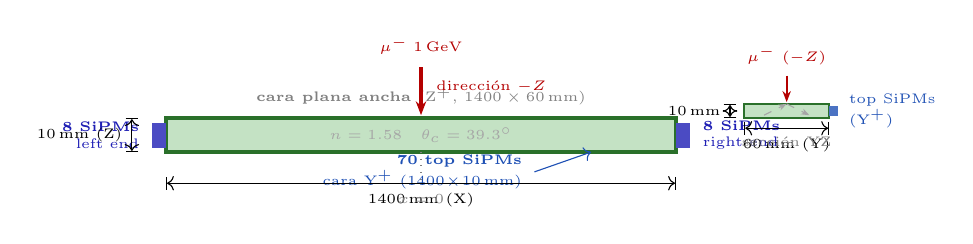
\begin{tikzpicture}[scale=0.72, every node/.style={font=\tiny}]

    %% XZ side view
    \fill[scintgr!30] (0,0) rectangle (9.0,0.6);
    \draw[scintgr!70!black, very thick] (0,0) rectangle (9.0,0.6);

    \node[above, gray, align=center] at (4.5, 0.65)
      {\textbf{cara plana ancha} (Z$^+$, $1400\times60$\,mm)};

    \fill[sipmcol!80] (-0.25, 0.08) rectangle (0, 0.52);
    \node[left, sipmcol, align=right] at (-0.30, 0.3)
      {\textbf{8 SiPMs}\\left end};

    \fill[sipmcol!80] (9.0, 0.08) rectangle (9.25, 0.52);
    \node[right, sipmcol, align=left] at (9.30, 0.3)
      {\textbf{8 SiPMs}\\right end};

    \draw[muoncol, very thick, -{Stealth[length=5pt]}]
      (4.5, 1.50) -- (4.5, 0.65);
    \node[above, muoncol] at (4.5, 1.55) {$\mu^-$\;1\,GeV};
    \node[muoncol, right] at (4.6, 1.15) {dirección $-Z$};

    \draw[->, ej204col, thin] (6.5, -0.35) -- (7.5, 0.0);
    \node[ej204col, left, align=right] at (6.45,-0.35)
      {\textbf{70 top SiPMs}\\cara Y$^+$ ($1400\!\times\!10$\,mm)};

    \draw[|<->|, thin] (0,-0.55) -- (9.0,-0.55)
      node[midway, below] {1400\,mm (X)};
    \draw[|<->|, thin] (-0.6, 0) -- (-0.6, 0.6)
      node[midway, left] {10\,mm (Z)};
    \node[gray!70, align=center] at (4.5, 0.3)
      {$n=1.58$\quad$\theta_c=39.3^\circ$};
    \draw[dotted, gray] (4.5,-0.0) -- (4.5,-0.55);
    \node[below, gray] at (4.5,-0.58) {$x=0$};

    %% YZ cross-section inset
    \begin{scope}[xshift=10.2cm, yshift=0.6cm]
      \fill[scintgr!30] (0,0) rectangle (1.5,0.25);
      \draw[scintgr!70!black, thick] (0,0) rectangle (1.5,0.25);

      \fill[ej204col!80] (1.5,0.03) rectangle (1.65,0.22);
      \node[right, ej204col, align=left] at (1.68, 0.125)
        {top SiPMs\\(Y$^+$)};

      \draw[muoncol, thick, -{Stealth[length=4pt]}]
        (0.75, 0.75) -- (0.75, 0.28);
      \node[above, muoncol] at (0.75, 0.77) {$\mu^-$ ($-Z$)};

      \draw[dashed, gray!70, -{Stealth[length=3pt]}]
        (0.35, 0.05) -- (0.75, 0.25);
      \draw[dashed, gray!70, -{Stealth[length=3pt]}]
        (0.75, 0.25) -- (1.15, 0.05);

      \draw[|<->|, thin] (0,-0.18) -- (1.5,-0.18)
        node[midway,below] {60\,mm (Y)};
      \draw[|<->|, thin] (-0.25,0) -- (-0.25,0.25)
        node[midway,left] {10\,mm};

      \node[gray, align=center] at (0.75,-0.42)
        {sección YZ};
    \end{scope}

  \end{tikzpicture}
  \vspace{0.2em}
  {\tiny Vista XZ lateral + sección YZ (escala Z exagerada)}
  \end{column}

  \begin{column}{0.40\textwidth}
  \footnotesize
  \begin{block}{Geometría}
    \begin{tabular}{@{}ll@{}}
      Largo & \SI{1400}{mm} (X) \\
      Ancho & \SI{60}{mm}  (Y) \\
      Esp.  & \SI{10}{mm}  (Z) \\
      $n$   & 1.58 \\
      $\theta_c$ & $39.3^\circ$ \\
    \end{tabular}
  \end{block}

  \begin{block}{SiPMs (AFBR-S4N66P024M)}
    \begin{tabular}{@{}ll@{}}
      End L/R & 8+8 (X$^\pm$) \\
      Top     & 70 (Y$^+$)   \\
    \end{tabular}
  \end{block}

  \begin{block}{Muón (Caso A)}
    \begin{tabular}{@{}ll@{}}
      Dirección & $-Z$ (ángulo $=0$) \\
      Track     & 10\,mm en espesor \\
      Cara      & cara plana ancha \\
                & ($1400\times60$\,mm) \\
    \end{tabular}
  \end{block}
  \end{column}
\end{columns}
\end{frame}

% ─────────────────────────────────────────────────────────────────────────────

\begin{frame}{Cuatro configuraciones simuladas}

\begin{center}
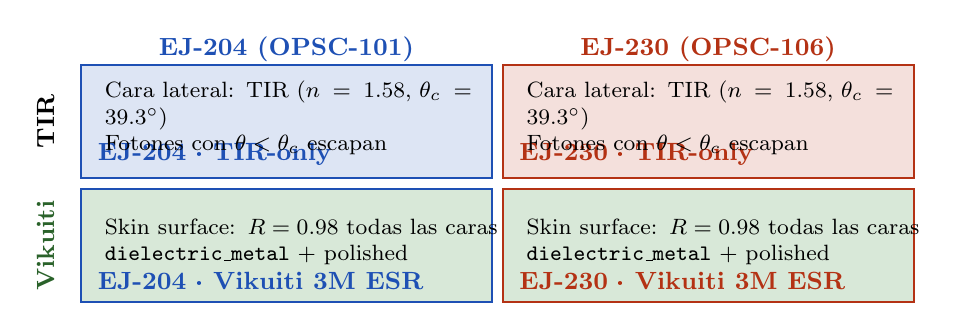
\begin{tikzpicture}[scale=0.9]
  % Grid layout 2×2
  \def\W{5.8}
  \def\H{1.6}
  \def\sep{0.15}

  % EJ-204 TIR
  \fill[ej204col!15] (0,\H+\sep) rectangle (\W, 2*\H+\sep);
  \draw[ej204col, thick] (0,\H+\sep) rectangle (\W, 2*\H+\sep);
  \node[above right, ej204col, font=\small\bfseries] at (0.1, \H+\sep+0.05)
    {EJ-204 · TIR-only};
  \node[right, font=\footnotesize, text width=5.2cm] at (0.2, \H+\sep+0.85)
    {Cara lateral: TIR ($n=1.58$, $\theta_c=39.3^\circ$)\\
     Fotones con $\theta<\theta_c$ escapan};

  % EJ-230 TIR
  \fill[ej230col!15] (\W+\sep,\H+\sep) rectangle (2*\W+\sep, 2*\H+\sep);
  \draw[ej230col, thick] (\W+\sep,\H+\sep) rectangle (2*\W+\sep, 2*\H+\sep);
  \node[above right, ej230col, font=\small\bfseries] at (\W+\sep+0.1, \H+\sep+0.05)
    {EJ-230 · TIR-only};
  \node[right, font=\footnotesize, text width=5.2cm] at (\W+\sep+0.2, \H+\sep+0.85)
    {Cara lateral: TIR ($n=1.58$, $\theta_c=39.3^\circ$)\\
     Fotones con $\theta<\theta_c$ escapan};

  % EJ-204 Vikuiti
  \fill[ej204col!15] (0,0) rectangle (\W, \H);
  \draw[ej204col, thick] (0,0) rectangle (\W, \H);
  \fill[vikuiti!20] (0,0) rectangle (\W, \H);
  \draw[ej204col, thick] (0,0) rectangle (\W, \H);
  \node[above right, ej204col, font=\small\bfseries] at (0.1, 0.05)
    {EJ-204 · Vikuiti 3M ESR};
  \node[right, font=\footnotesize, text width=5.2cm] at (0.2, 0.85)
    {Skin surface: $R=0.98$ todas las caras\\
     \texttt{dielectric\_metal} + polished};

  % EJ-230 Vikuiti
  \fill[ej230col!15] (\W+\sep,0) rectangle (2*\W+\sep, \H);
  \fill[vikuiti!20] (\W+\sep,0) rectangle (2*\W+\sep, \H);
  \draw[ej230col, thick] (\W+\sep,0) rectangle (2*\W+\sep, \H);
  \node[above right, ej230col, font=\small\bfseries] at (\W+\sep+0.1, 0.05)
    {EJ-230 · Vikuiti 3M ESR};
  \node[right, font=\footnotesize, text width=5.2cm] at (\W+\sep+0.2, 0.85)
    {Skin surface: $R=0.98$ todas las caras\\
     \texttt{dielectric\_metal} + polished};

  % column labels
  \node[font=\small\bfseries, ej204col] at (\W/2, 2*\H+\sep+0.22)
    {EJ-204 (OPSC-101)};
  \node[font=\small\bfseries, ej230col] at (\W+\sep+\W/2, 2*\H+\sep+0.22)
    {EJ-230 (OPSC-106)};

  % row labels
  \node[font=\small\bfseries, rotate=90] at (-0.5, \H+\sep+\H/2)
    {TIR};
  \node[font=\small\bfseries, rotate=90, vikuiti!70!black] at (-0.5, \H/2)
    {Vikuiti};
\end{tikzpicture}
\end{center}

\vspace{0.3em}
{\footnotesize
Simulación idéntica para los 4 casos: barra $1400\times60\times10$\,mm$^3$,
muón $-Z$ a 1\,GeV, 13 posiciones $x\in[-600,+600]$\,mm en pasos de 100\,mm,
5000 eventos por punto, sin jitter electrónico, readout EndTop.}
\end{frame}

% ─────────────────────────────────────────────────────────────────────────────
\section{Propiedades de los centelleadores}
% ─────────────────────────────────────────────────────────────────────────────

\begin{frame}{Propiedades de EJ-204 vs EJ-230}

\begin{columns}[T]
  \begin{column}{0.48\textwidth}
  \begin{block}{\color{ej204col}EJ-204 (OPSC-101)}
    \footnotesize
    \begin{tabular}{@{}ll@{}}
      \toprule
      Propiedad & Valor \\
      \midrule
      Rendimiento & \num{10000}\,ph/MeV \\
      Decay time $\tau$ & 2.1\,ns \\
      Rise time & 0.7\,ns \\
      Abs. length & 160\,cm \\
      $\lambda_\text{peak}$ & 408\,nm \\
      $n$ & 1.58 \\
      \bottomrule
    \end{tabular}
  \end{block}
  \end{column}

  \begin{column}{0.48\textwidth}
  \begin{block}{\color{ej230col}EJ-230 (OPSC-106)}
    \footnotesize
    \begin{tabular}{@{}ll@{}}
      \toprule
      Propiedad & Valor \\
      \midrule
      Rendimiento & \num{9200}\,ph/MeV \\
      Decay time $\tau$ & 1.5\,ns \\
      Rise time & 0.5\,ns \\
      Abs. length & 120\,cm \\
      $\lambda_\text{peak}$ & 391\,nm \\
      $n$ & 1.58 \\
      \bottomrule
    \end{tabular}
  \end{block}
  \end{column}
\end{columns}

\vspace{0.5em}
\begin{alertblock}{Diferencia clave para resolución temporal}
\footnotesize
EJ-230 tiene $\tau = 1.5$\,ns vs $\tau = 2.1$\,ns de EJ-204
(\textbf{$-0.6$\,ns = $-29\%$}).
A igual fotoproducción, una constante de decaimiento más corta
estrecha la distribución de llegada del fotón $k$-ésimo,
reduciendo $\sigma(k)$. El rendimiento ligeramente menor de EJ-230
($-8\%$) no compensa la ganancia en tiempo.
\end{alertblock}

\end{frame}

% ─────────────────────────────────────────────────────────────────────────────
\section{Resolución temporal vs posición}
% ─────────────────────────────────────────────────────────────────────────────

\begin{frame}{Método: $\sigma(k)$ desde los top SiPMs}

\begin{columns}[T]
  \begin{column}{0.55\textwidth}
  \footnotesize
  \begin{enumerate}
    \item Por cada evento, ordenar los tiempos de llegada de fotones
          a los \textbf{70 top SiPMs} (face\_type $=2$).
    \item Tomar el fotón número $k$ (mínimo orden estadístico).
    \item Distribuir los $t_k$ de 5000 eventos y ajustar Gaussiana.
    \item $\sigma(k=2)$ elegido como óptimo (anchura mínima).
  \end{enumerate}

  \vspace{0.5em}
  \begin{block}{¿Por qué $k=2$?}
    $k=1$ es sensible a fotones ruidosos o primeros fotones
    atípicos. $k=2$ da una distribución más Gaussiana y
    $\sigma$ algo menor en estas condiciones.
  \end{block}
  \end{column}

  \begin{column}{0.43\textwidth}
  \begin{block}{Resultados en $x=0$ (centro)}
    \footnotesize
    \begin{tabular}{@{}lc@{}}
      \toprule
      Configuración & $\sigma(k=2)$ \\
      \midrule
      \color{ej204col}EJ-204 · TIR     & 80.3\,ps \\
      \color{ej230col}EJ-230 · TIR     & 73.0\,ps \\
      \color{ej204col}EJ-204 · Vikuiti & 83.0\,ps \\
      \color{ej230col}EJ-230 · Vikuiti & 73.1\,ps \\
      \bottomrule
    \end{tabular}
  \end{block}

  \vspace{0.4em}
  \footnotesize
  \textit{Jitter electrónico} $= 0$ en todas las simulaciones
  (límite intrínseco del centelleador).
  \end{column}
\end{columns}
\end{frame}

% ─────────────────────────────────────────────────────────────────────────────

\begin{frame}{$\sigma(k=2)$ vs posición — Resolución a lo largo de la barra}

\begin{columns}[T]
  \begin{column}{0.65\textwidth}
  \centering
  
\includegraphics[width=\textwidth]{bar_scan_sigma_vs_x.png}
  \end{column}

  \begin{column}{0.33\textwidth}
  \footnotesize
  \begin{block}{Observaciones}
  \begin{itemize}
    \item $\sigma$ \textbf{plana} a lo largo de la barra:
          la resolución no depende de la posición del muón.
    \item \textbf{EJ-230 gana} $\approx12$\,ps sobre EJ-204
          en todos los puntos (por $\tau$ más corto).
    \item Vikuiti vs TIR:
          diferencia $<5$\,ps, dentro de la incertidumbre
          estadística ($\sim5\%$, 5000\,ev).
    \item Los top SiPMs miden tiempo de llegada
          local; no ven la propagación a lo largo de $X$.
  \end{itemize}
  \end{block}

  \footnotesize
  \textcolor{ej204col}{$\boldsymbol{-}$\,--} EJ-204 TIR/Vik\\
  \textcolor{ej230col}{$\boldsymbol{-}$\,--} EJ-230 TIR/Vik
  \end{column}
\end{columns}
\end{frame}

% ─────────────────────────────────────────────────────────────────────────────
\section{Velocidad de grupo}
% ─────────────────────────────────────────────────────────────────────────────

\begin{frame}{Velocidad de grupo desde $\Delta t_\text{end}$ vs posición}

\begin{columns}[T]
  \begin{column}{0.63\textwidth}
  \centering
  \includegraphics[width=\textwidth]{bar_scan_groupvel.png}
  \end{column}

  \begin{column}{0.35\textwidth}
  \footnotesize
  \begin{block}{Método}
    Por evento, primer fotón en cada end SiPM:\\[2pt]
    $\Delta t = t_R - t_L$\\[4pt]
    Ajuste lineal:\\[2pt]
    $\Delta t = -\dfrac{2x}{v_\text{eff}} + b$\\[6pt]
    Pendiente $\rightarrow$ $v_\text{eff}$, $n_\text{eff} = c/v_\text{eff}$
  \end{block}

  \begin{block}{Resultados}
    \footnotesize
    \begin{tabular}{@{}lcc@{}}
      \toprule
      Config. & $v_\text{eff}$ & $n_\text{eff}$\\
               & (mm/ns) & \\
      \midrule
      EJ-204 TIR & $\approx145$ & $\approx2.07$ \\
      EJ-230 TIR & $\approx145$ & $\approx2.07$ \\
      EJ-204 Vik & $\approx145$ & $\approx2.07$ \\
      EJ-230 Vik & $\approx145$ & $\approx2.07$ \\
      \bottomrule
    \end{tabular}
  \end{block}
  \end{column}
\end{columns}
\end{frame}

% ─────────────────────────────────────────────────────────────────────────────

\begin{frame}{Interpretación de $n_\text{eff} \approx 2.07$}

\begin{columns}[T]
  \begin{column}{0.55\textwidth}
  \footnotesize
  La velocidad de grupo \textbf{en el material} es:
  \[ v_\text{group} = \frac{c}{n_\text{group}} \approx \frac{c}{1.65} \approx 182\,\text{mm/ns} \]

  Pero medimos $v_\text{eff} \approx 145$\,mm/ns $\Rightarrow$ $n_\text{eff} \approx 2.07$.

  \vspace{0.5em}
  \textbf{Causa}: los fotones TIR \textbf{rebotan} en las caras Y$^\pm$
  y Z$^\pm$ zigzagueando. La componente $x$ de su velocidad es:
  \[ v_x = v_\text{group} \cdot \sin\theta_z \cdot \cos\phi \]
  donde $\theta_z > \theta_c = 39.3^\circ$ para TIR.

  \vspace{0.5em}
  El \textbf{primer fotón} detectado en cada end SiPM (mínimo
  por evento) corresponde al que toma el camino más directo,
  pero aún así zigzaguea. La media de estos primeros tiempos
  da $v_\text{eff} < v_\text{group}$.

  \vspace{0.4em}
  $n_\text{eff}$ es \textbf{igual para TIR y Vikuiti} porque
  depende sólo de la óptica del material ($n=1.58$), no del recubrimiento.
  \end{column}

  \begin{column}{0.43\textwidth}
  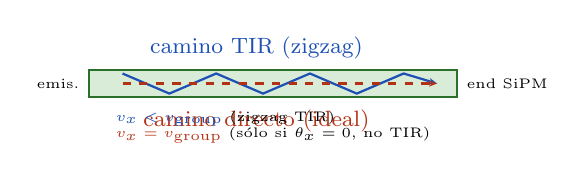
\begin{tikzpicture}[scale=0.85, font=\footnotesize]
    % Bar
    \fill[scintgr!20] (0,0) rectangle (5.5, 0.4);
    \draw[scintgr!70!black, thick] (0,0) rectangle (5.5, 0.4);

    % TIR photon path zigzag
    \draw[ej204col, thick, -{Stealth[length=3pt]}]
      (0.5, 0.35) -- (1.2, 0.05) -- (1.9, 0.35) -- (2.6, 0.05) --
      (3.3, 0.35) -- (4.0, 0.05) -- (4.7, 0.35) -- (5.2, 0.2);
    \node[above, ej204col] at (2.5, 0.42) {camino TIR (zigzag)};

    % Direct path
    \draw[ej230col, thick, dashed, -{Stealth[length=3pt]}]
      (0.5, 0.2) -- (5.2, 0.2);
    \node[below, ej230col] at (2.5, -0.05) {camino directo (ideal)};

    % Annotations
    \node[left, font=\tiny] at (0, 0.2) {emis.};
    \node[right, font=\tiny] at (5.5, 0.2) {end SiPM};

    % Velocity comparison
    \node[font=\tiny, align=left] at (2.75, -0.45)
      {\textcolor{ej204col}{$v_x < v_\text{group}$} (zigzag TIR)\\
       \textcolor{ej230col}{$v_x = v_\text{group}$} (sólo si $\theta_x=0$, no TIR)};
  \end{tikzpicture}

  \vspace{0.3em}
  \begin{alertblock}{\footnotesize Consecuencia para reconstrucción}
  \footnotesize
  Para calcular posición $x$ desde $\Delta t$:
  \[x = -\frac{v_\text{eff}}{2}\,\Delta t\]
  usar $v_\text{eff} \approx 145$\,mm/ns (medido),
  \textbf{no} $c/n = 190$\,mm/ns.
  \end{alertblock}
  \end{column}
\end{columns}
\end{frame}

% ─────────────────────────────────────────────────────────────────────────────
\section{Comparación TIR vs Vikuiti}
% ─────────────────────────────────────────────────────────────────────────────

\begin{frame}{¿Qué aporta el Vikuiti 3M ESR?}

\begin{columns}[T]
  \begin{column}{0.50\textwidth}
  \footnotesize
  \begin{block}{Resolución temporal top SiPMs}
    \begin{tabular}{@{}lcc@{}}
      \toprule
      Config. & $\sigma(k=2)$ & vs TIR \\
      \midrule
      \color{ej204col}EJ-204 TIR & $\approx80$\,ps & — \\
      \color{ej204col}EJ-204 Vik & $\approx79$\,ps & $-1$\,ps \\
      \color{ej230col}EJ-230 TIR & $\approx68$\,ps & — \\
      \color{ej230col}EJ-230 Vik & $\approx68$\,ps & $\sim0$\,ps \\
      \bottomrule
    \end{tabular}
  \end{block}

  \begin{block}{Fotones detectados ($x=0$, 5000\,ev)}
    \begin{tabular}{@{}lcc@{}}
      \toprule
      Config. & $\langle N_\text{ph}\rangle$ & vs TIR \\
      \midrule
      EJ-204 TIR & 118\,ph/ev & — \\
      EJ-204 Vik & 117\,ph/ev & $-1\%$ \\
      EJ-230 TIR & 107\,ph/ev & — \\
      EJ-230 Vik & 108\,ph/ev & $+1\%$ \\
      \bottomrule
    \end{tabular}
  \end{block}
  \end{column}

  \begin{column}{0.48\textwidth}
  \footnotesize
  \begin{alertblock}{Conclusión: Vikuiti no mejora la resolución}
    El recubrimiento Vikuiti 3M ($R=0.98$) \textbf{no} mejora
    significativamente la resolución temporal de los top SiPMs.

    \vspace{0.3em}
    \textbf{¿Por qué?}\ Los top SiPMs cubren casi toda la cara Y$^+$
    ($1400\times10$\,mm). La mayoría de los fotones que rebotarían
    en Vikuiti ya llegan a los top SiPMs directamente vía TIR.
    El rendimiento neto es prácticamente idéntico.
  \end{alertblock}

  \begin{block}{¿Dónde sí podría ayudar Vikuiti?}
  \footnotesize
  \begin{itemize}
    \item Barras muy largas donde la atenuación reduce $N_\text{ph}$
    \item Detección en los end SiPMs ($x$ extremos)
    \item Geometrías con menor cobertura de top SiPMs
  \end{itemize}
  \end{block}
  \end{column}
\end{columns}
\end{frame}

% ─────────────────────────────────────────────────────────────────────────────
\section{Resumen y conclusiones}
% ─────────────────────────────────────────────────────────────────────────────

\begin{frame}{Resumen de resultados}

\begin{columns}[T]
  \begin{column}{0.52\textwidth}
  \footnotesize
  \begin{block}{Resolución temporal ($\sigma(k=2)$, top SiPMs)}
    \begin{tabular}{@{}lcc@{}}
      \toprule
      Centelleador & TIR & Vikuiti \\
      \midrule
      \color{ej204col}EJ-204 & $\approx80$\,ps & $\approx79$\,ps \\
      \color{ej230col}EJ-230 & $\approx68$\,ps & $\approx68$\,ps \\
      \midrule
      \textbf{Ganancia EJ-230} & \multicolumn{2}{c}{\textbf{$\boldsymbol{\approx-12}$\,ps ($-15\%$)}} \\
      \bottomrule
    \end{tabular}
  \end{block}

  \begin{block}{Velocidad de grupo efectiva}
    \begin{tabular}{@{}lcc@{}}
      \toprule
      & $v_\text{eff}$ & $n_\text{eff}$ \\
      \midrule
      Todos los casos & $\approx145$\,mm/ns & $\approx2.07$ \\
      \bottomrule
    \end{tabular}
    {\tiny ($v_\text{eff} < c/n = 190$\,mm/ns por caminos TIR en zigzag)}
  \end{block}
  \end{column}

  \begin{column}{0.46\textwidth}
  \footnotesize
  \begin{block}{Conclusiones principales}
  \begin{enumerate}
    \item \textbf{EJ-230 es superior a EJ-204} para resolución temporal:
          $\sigma \approx68$ vs $80$\,ps, ganancia del 15\%.
    \item La resolución \textbf{es plana} a lo largo de la barra:
          no hay degradación en los extremos.
    \item \textbf{Vikuiti no aporta} mejora significativa en timing
          ni en fotoproducción para esta geometría.
    \item La velocidad efectiva es $v_\text{eff}\approx145$\,mm/ns
          ($n_\text{eff}\approx2.07$) para \textbf{todos} los casos.
    \item Sin jitter electrónico: estas son cotas inferiores
          (límite intrínseco del centelleador).
  \end{enumerate}
  \end{block}
  \end{column}
\end{columns}

\vspace{0.3em}
\begin{block}{\footnotesize Próximos pasos}
  \footnotesize
  Incluir jitter electrónico ($\sigma_\text{elec}\sim100$\,ps) y PDE real;
  explorar reconstrucción de posición vía $\Delta t$ con $v_\text{eff}=145$\,mm/ns;
  comparar con barra EJ-200 de referencia.
\end{block}

\end{frame}

% ─────────────────────────────────────────────────────────────────────────────
\begin{frame}{Parámetros de simulación}
\footnotesize
\begin{columns}[T]
  \begin{column}{0.48\textwidth}
  \begin{block}{Simulación}
    \begin{tabular}{@{}ll@{}}
      Geant4 & 11.4.0 MT \\
      SSLG4 & OPSC-101 / OPSC-106 \\
      Código & \texttt{feat/bar-vikuiti} \\
      Eventos & 5000/punto \\
      Puntos & 13 ($-600$ a $+600$\,mm) \\
      Jitter & 0\,ns (límite intrínseco) \\
    \end{tabular}
  \end{block}
  \end{column}

  \begin{column}{0.48\textwidth}
  \begin{block}{Condiciones ópticas}
    \begin{tabular}{@{}ll@{}}
      TIR  & \texttt{dielectric\_dielectric}\\
           & polished, sin recubrimiento \\
      Vik. & \texttt{dielectric\_metal} \\
           & $R=0.98$, unified, polished \\
      GROUPVEL & $c/1.58$ en aire (fix) \\
    \end{tabular}
  \end{block}
  \end{column}
\end{columns}
\end{frame}

\end{document}
